\documentclass[12pt]{ctexart}
\usepackage{geometry}       % 设置页面整体布局
\geometry{top=2.5cm, bottom=2.5cm, left=2cm, right=2cm}
\usepackage{fancyhdr}       % 设置页眉页脚布局
\pagestyle{fancy}
\rhead{\thepage}            % 设置右页眉为页数
\chead{中国科学技术大学}
\cfoot{}                    % 设置中间页脚为空
\usepackage{amsmath}        % 数学公式宏包
\numberwithin{equation}{section}
\usepackage{esint}          % 交叉引用宏包
\usepackage[colorlinks,     % 设置引用的颜色
            linkcolor=black,
            anchorcolor=black,
            urlcolor=cyan,
            citecolor=black,
           ]{hyperref}
\usepackage{makecell}       % 插入表格宏包
\usepackage{longtable}      % 长表格宏包
\usepackage{appendix}       % 生成附录宏包
\usepackage{graphicx}       % 插入图片宏包
\usepackage{epstopdf}       % 插入eps图片宏包
\usepackage{cite}           % 文献引用宏包
\renewcommand{\thefigure}   % 设置图片编号格式
    {\thesection{}.\arabic{figure}}
\renewcommand{\thefootnote}{} % 设置角标编号不出现在文中
                            % 以\footnotetext{Footnotetext without footnote mark}使用
\usepackage{unicode-math}
\usepackage{listings}
\usepackage{hyperref}



\CTEXsetup[format={\Large\bfseries}]{section}

\begin{document}

\nocite{*}

\begin{center}
    \heiti \fontsize{24pt}{0}{恒温槽的装配与性能测定}

    \vspace{12pt}

    \kaishu \fontsize{13.75pt}{0}禤科材
    

    \footnotetext{\textbf{实验日期:}2022年11月25日}
    \footnotetext{\textbf{作者简介:}禤科材(2002-),男,学号PB20030874,中国科学技术大学本科在读,专业方向为化学物理}
    \footnotetext{\textbf{联系方式:}电话 18108064415 ,邮箱 \href{mailto:ustcxkc@mail.ustc.edu.cn}{ustcxkc@mail.ustc.edu.cn}}

    \vspace{5pt}

    \songti \fontsize{12pt}{0}(中国科学技术大学化学与材料科学学院,安徽 合肥 230026)
\end{center}

\noindent\textbf{摘~~~\!要}~~~\!
恒温槽是物理化学实验中一个非常重要的装置,它可以保持物理化学反应在
一个相对恒定的温度下进行。恒温槽的温度控制有很多种方法,在本实验中,
通过绘制温度-时间曲线,研究了 DTC 控温仪和电磁继电器两种控温装置对
控温效果的影响,以及电压、冷凝水等外部条件对恒温槽控制效果的影响,
从而便于其在未来其他物理化学实验中正确的应用。
\newline
\textbf{关键字}~~~\!
恒温槽;DTC 控温仪;电磁继电器

\begin{center}
    {\LARGE\rmfamily\textbf{Assembling and Performance Determination of Thermostatic Bath}}

    \vspace{12pt}

    {\slshape Xuan Kecai}

    \vspace{5pt}

    (School of Chemistry and Material Science, USTC, Hefei 230026, China)
\end{center}

\noindent\textbf{Abstract}~~~\!
Constant temperature bath is a very important device in
physical and chemical experiments, which can keep physical
and chemical reactions at a relatively constant temperature.
There are many ways to control the temperature of a constant
temperature bath. In this experiment, by drawing a
temperature-time curve, the influence of two temperature
control devices, DTC temperature controller and
electromagnetic relay, on the temperature control effect, as
well as external voltage, condensate, etc. The influence of
conditions on the control effect of the constant temperature
bath, so as to facilitate its correct application in other
physical and chemical experiments in the future.
\newline
\textbf{Keywords}~~~\!
Thermostatic bath; DTC thermostat; Electromagnetic relay

\section{序言}

恒温装置是物理化学实验中一个非常重要的装置。在实验测量与温度有关的
物理量例如折射率、粘度、电导、蒸汽压、电动势、化学反应的速率常数、
电离平衡常数时$^{[1]}$,我们都会用到恒温装置。恒温槽是一种常见的
恒温装置。恒温槽通过控制浴液温度的恒定来达到恒温效果。利用恒温槽
可以保持实验环境温度的相对稳定。提高恒温槽的控制精度则可以有效减少
由于温差引起的实验误差。

恒温槽包括敏感元件、控制元件和加热元件三部分,三者相互配合控制
恒温槽的温度处于一个较小的区间。通过作温度$\sim$时间图像可以得到的
各个条件下的温差$\sim$时间曲线,假设温度差曲线的最大值为$t_1$,
最小值为$t_2$,则恒温槽的灵敏度为
\begin{align}
    t = \pm \frac{t_1 - t_2}{2}.
\end{align}

本实验比较了不同实验设备对温度控制的效果。

\section{实验}
\subsection{试剂与仪器}

自来水。

DTC-2AI 控温仪(南京南大万和科技有限公司)、DHJF-2005 型低温恒温
搅拌反应浴(郑州长城科工贸有限公司)、HK-2A 超级恒温水浴(南京南大
万和科技有限公司)、NTY-10A 型数字式千分温度计(南京南大万和科技
有限公司)、电磁继电器、接触温度计、TDGC2-3KVA 型接触调压器(上海
全力电器有限公司)。

\subsection{实验方法}
\subsubsection{不通冷凝水时恒温槽灵敏度的测定}

测定超级恒温水浴在 30$^\circ$C 附近的温度变化,打开精密电子温差
测量仪,使用 DTC 控制,将变电器电压调至 125 V,记录数据;再将电压
调至 200 V,记录数据。然后变动开关,使用电子继电器控制,将变压器
电压调至 125 V,记录数据;再将电压调至 200 V,记录数据。

\subsubsection{通入冷凝水时恒温槽灵敏度的测定}

打开阀门,向恒温槽中通入 30$^\circ$C 左右的冷凝水,重复 2.2.1 节
中的实验操作。

\section{结果分析与讨论}
\subsection{实验结果展示}

所有八组实验结果如图 3.1 所示。各组实验数据的单张图片见附件。

\begin{figure}[!h]
    \centering
    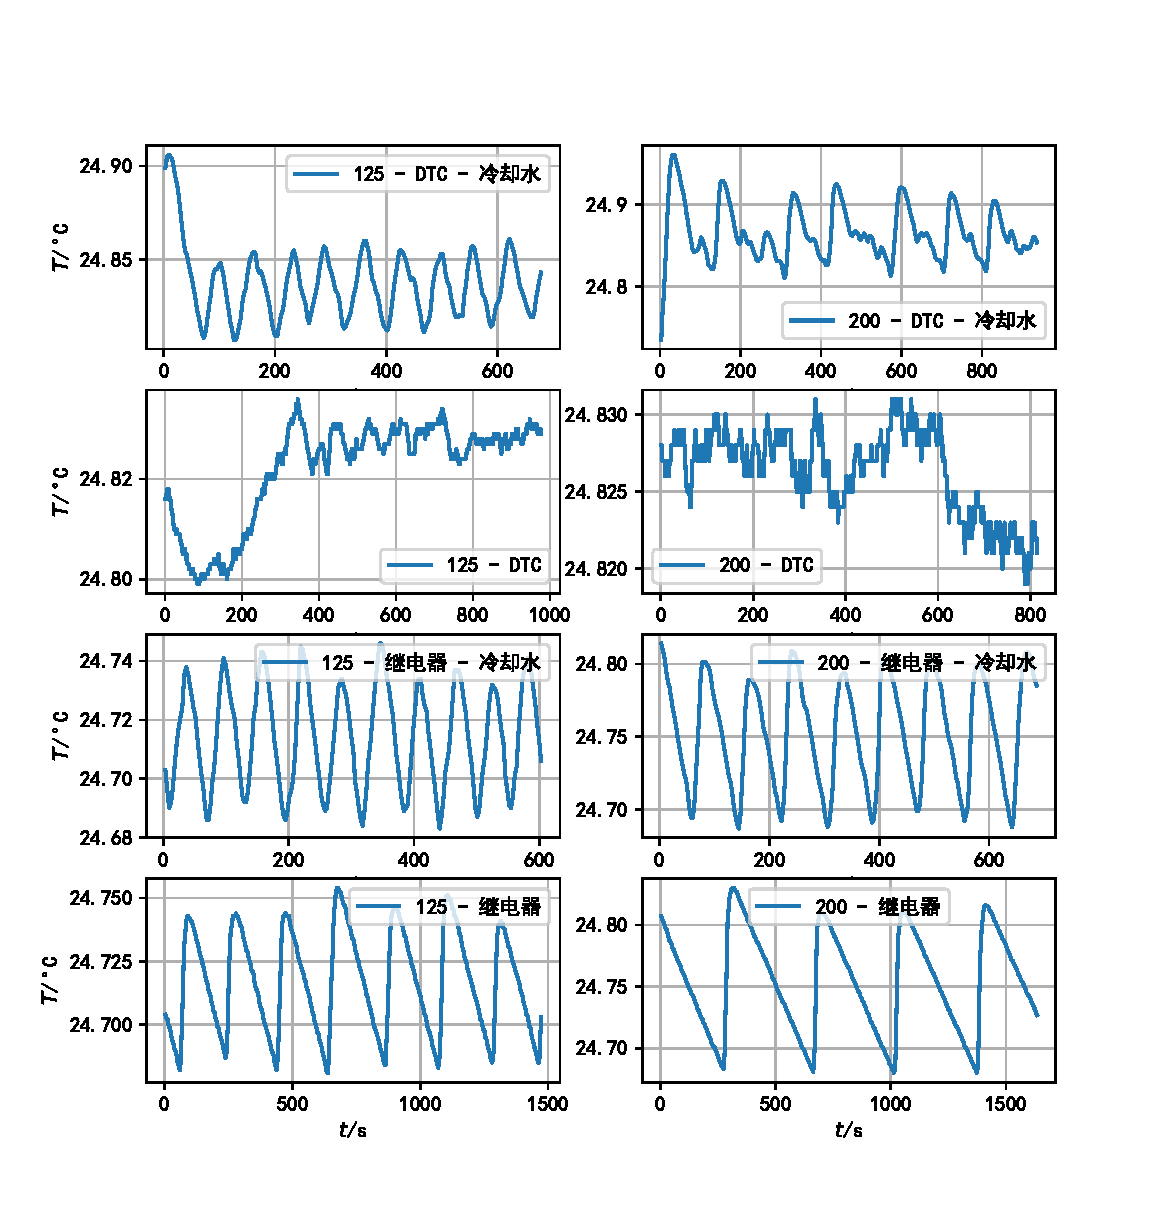
\includegraphics[scale=0.88]{plot_all.pdf}
    \caption{总实验结果}
\end{figure}

\subsection{实验数据分析}

计算不同实验条件下的平均温度$\overline{T}$,装置控温的灵敏度$t$
以及控温周期。八组实验的计算结果如表 1 所示。其中 125 V-DTC
控制-通冷却水组的实验数据取 100 s $\sim$ 600 s 的数据进行处理;
200 V-DTC 控制-通冷却水组的实验数据取 100 s $\sim$ 900 s 的数据
进行处理; 125 V-DTC控制-无冷却水组的实验数据取 400 s $\sim$
900 s 的数据进行处理;200 V-DTC 控制-无冷却水组的实验数据取 0 s
$\sim$ 600 s 的数据进行处理;其他组取全时间段的数据进行处理。

\begin{longtable}{ccccccc}
    \caption{实验数据处理表格} \\
    \hline
    组别 & 控制器 & 电压/V & 是否通冷凝水 & 平均温度/$^\circ$C
        & 灵敏度/$^\circ$C & 周期/s \\
    \hline
    1 & DTC & 125 & 否 & 24.80 & $\pm3.00\times 10^{-03}$& 73 \\
    2 & DTC & 200 & 否 & 24.83 & $\pm2.00\times 10^{-03}$ & 无明显周期 \\
    3 & DTC & 125 & 是 & 24.83 & $\pm2.30\times 10^{-02}$ & 63 \\
    4 & DTC & 200 & 是 & 24.86 & $\pm5.60\times 10^{-02}$ & 116 \\
    5 & 继电器 & 125 & 否 & 24.72 & $\pm3.10\times 10^{-02}$ & 174 \\
    6 & 继电器 & 200 & 否 & 24.75 & $\pm4.30\times 10^{-02}$ & 237 \\
    7 & 继电器 & 125 & 是 & 24.72 & $\pm2.90\times 10^{-02}$ & 54 \\
    8 & 继电器 & 200 & 是 & 24.76 & $\pm5.65\times 10^{-02}$ & 83 \\
    \hline
\end{longtable}

\subsubsection*{相同条件-不同加热电压}

由数据处理结果表格可以看出,在高加热电压(200V)条件下,体系的平均
温度比低电压条件(125V)下的平均温度更高。高电压下控温装置的
周期更长,灵敏度更低(温度波动范围更大)。

由于实验时恰逢降温,天气较冷,故高电压时体系的平均
温度更加接近实验设置的 30 $^\circ$C,不过实验记录距离竟有 5 $^\circ$C 之差,可能是仪器未校准或是
数据传输的原因,不过并不影响本实验对恒温装置灵敏性与可靠性的判断。

\subsubsection*{相同条件-是否通冷却水}

由数据处理结果表格可以看出,在相同条件下,通冷却水时体系的平均温度
略有上升,控温装置的控温周期显著缩短,灵敏度略有降低(温度波动范围
更大)。

通冷却水模拟的是更高设定温度的实验条件。由此可以得出一些推论,
若实验设定的目标温度更高,将有如下结果:(1)体系的平均温度将会
上升,这是显然的,因为设定温度升高了;(2)控温装置的周期将会缩短,
这说明控温系统需要更加频繁的进行加热和断电以控制恒温,这是因为散热
速度会变快,因此系统需要更频繁的加热;(3)控温的灵敏度将会下降,
即温度的波动将会更大,这是因为系统的散热会更加剧烈,因此温度波动会
更加剧烈。

\subsubsection*{相同条件-不同控温装置}

由数据处理结果表格可以看出,在相同条件下,用 DTC 控温时体系的平均
温度显著高于用继电器控制的平均温度,且更加接近设定的目标温度。
DTC 控温的灵敏度显著高于继电器装置。不通冷却水时,DTC 控温的周期
更长;通冷却水时,继电器控温的周期更长。

DTC 控温系统使用四个参数控制 PID 三个控温参数。PID 参数分别表示
过去温度的影响、温度的积分影响和温度的微分影响。而继电器控温系统仅
依靠当前温度值进行“通路”和“断路”的判断,这种判断具有滞后性,受诸多
环境因素影响。因此 DTC 控温系统全方位控制温度,比用继电器实现的
仅靠当前温度进行的控温效果要更好。因而 DTC 控温的体系平均温度更
接近于设定的温度,控温灵敏度更高。

\subsection{提高灵敏度的方法}

(1)加大搅拌功率:由扩散传质方程可知,搅拌对流越剧烈,热量传导
越快。传热速度加快,加热的滞后效应就越弱,控温装置的灵敏度就越高。

(2)设置合适的加热功率:若加热功率过高,会使加热的滞后效应更加
明显,灵敏度会降低;若加热功率过低,会使系统接受的热量过少,导致
灵敏度下降,甚至无法达到恒温目标。

(3)选用合理的介质:介质的沸点应比目标温度高。在此基础上,介质
的粘度应该尽量小,这样介质易于流动,搅拌效果更好,灵敏度更高;同时
介质的比热容应该尽量大,这样吸收或放出相同的热量时介质的温度变化
更小,更易于控温装置精密调节温度,灵敏度高。

(4)合理排布部件位置:在恒温槽中,加热部件应与搅拌装置放在一起,
这样会减少热量的累计,减弱加热时的滞后效应,提高装置的灵敏度。
同时感温装置与加热部件的距离应选择合适的值,若距离太近,则测得的
温度偏高;若距离太远,则测得的温度会偏低。这都不利于温度的控制。
另外,恒温槽中的装置都不应放在槽的角落位置。由流体力学原理可知,
与器壁相靠近的位置的液体流速受搅拌对流的影响小,若有器件放在此处,
则搅拌装置无法对其起到较好的效果,会造成灵敏度的降低。

\subsection{误差分析}

(1)感温部件是本实验最关键的部分之一,其测量的准确度直接影响了
控温装置的控制效果以及得到的数据的准确性。其误差是本实验误差的主要
来源。在使用触点式温度控制装置时,需要人工调节接触温度计中金属丝的
位置以设定恒温温度,该操作有较大误差。

(2)由于热量的传导需要时间,而整个实验又是在不断的加热-散热过程中
进行。因此体系的温度时刻在发生变化,不同位置测得的温度并不相同,
从而导致了一定的实验误差。

(3)室内温度的波动对于更为敏感的精密恒温控制装置影响较为明显,
且空气流动等也会影响其准确性,我们从图中可以明显看出散热速率大、
加热电压小的精密恒温控制装置的一个周期内也有极值点的出现,这很可能
是室温波动和空气流动导致的。

\section{结语}

本实验研究了 DTC 和继电器两种控制温度的方法的区别,通过实验,DTC
控制温度的效果要明显优于继电器控制。同一控制器下,低电压下的恒温槽
灵敏度优于高电压的灵敏度,而由于升温幅度大,继电器在高压下温度
变化的周期更长,同时通入冷凝水也会降低控温装置的灵敏度。

\begin{center}
    \Large\bfseries{参考文献}
\end{center}
\noindent
[1] 傅献彩, 沈文霞, 姚天扬等. 物理化学(第五版). 上册[M].
高等教育出版社,2006.

\newpage

\begin{center}
    \LARGE\bfseries{附件~~~实验数据处理}
\end{center}
\begin{center}
    \Large\bfseries{附件I~~~实验图像处理}
\end{center}

\begin{figure}[!h]
    \centering
    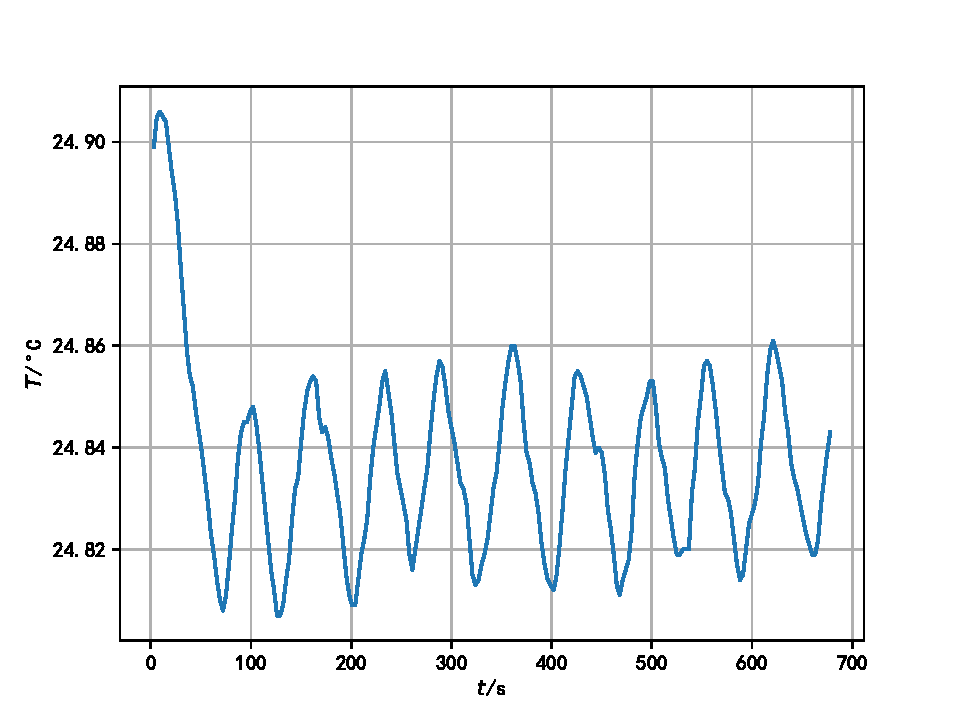
\includegraphics[scale=0.68]{Figure_1.pdf}
    \caption{DTC 控制,电压125 V,通冷却水}
\end{figure}

\begin{figure}[!h]
    \centering
    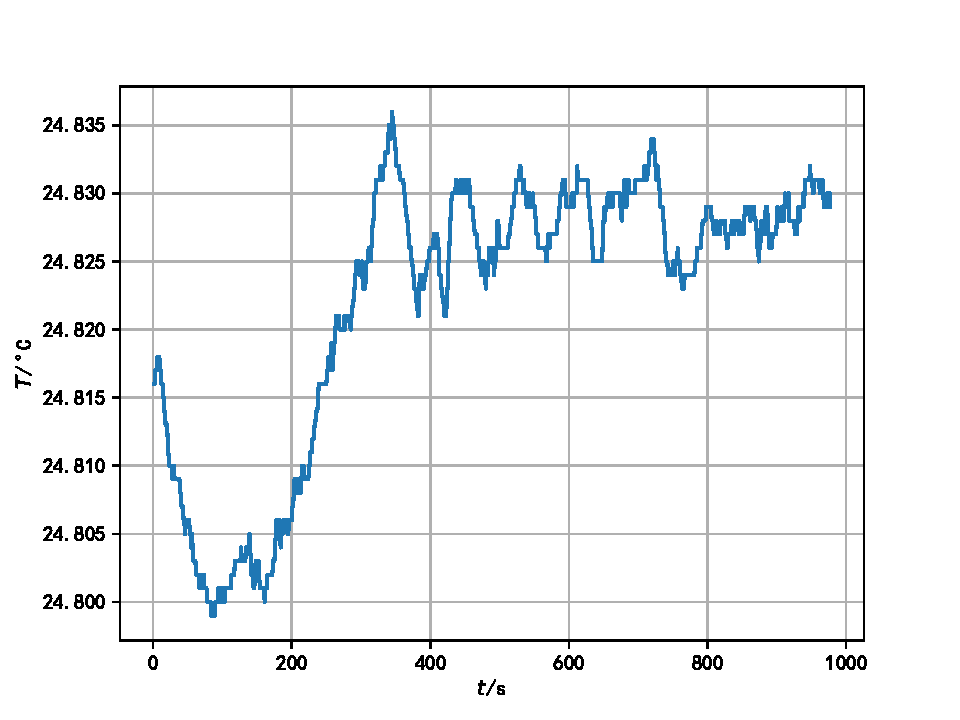
\includegraphics[scale=0.68]{Figure_2.pdf}
    \caption{DTC 控制,电压125 V,未通冷却水}
\end{figure}

\begin{figure}[!h]
    \centering
    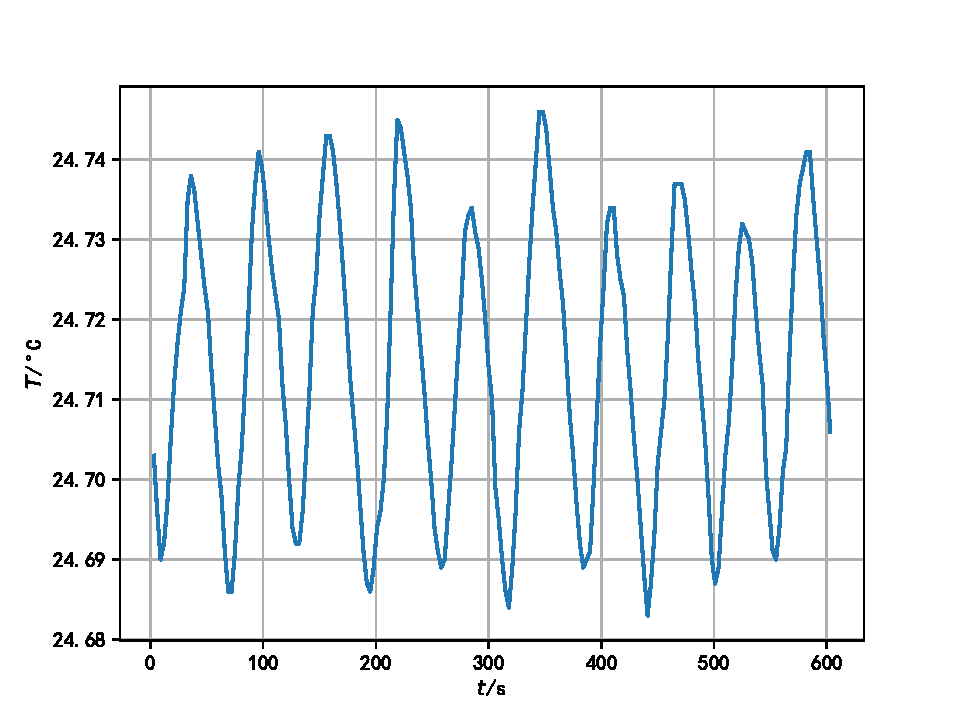
\includegraphics[scale=0.68]{Figure_3.pdf}
    \caption{继电器控制,电压125 V,通冷却水}
\end{figure}

\begin{figure}[!h]
    \centering
    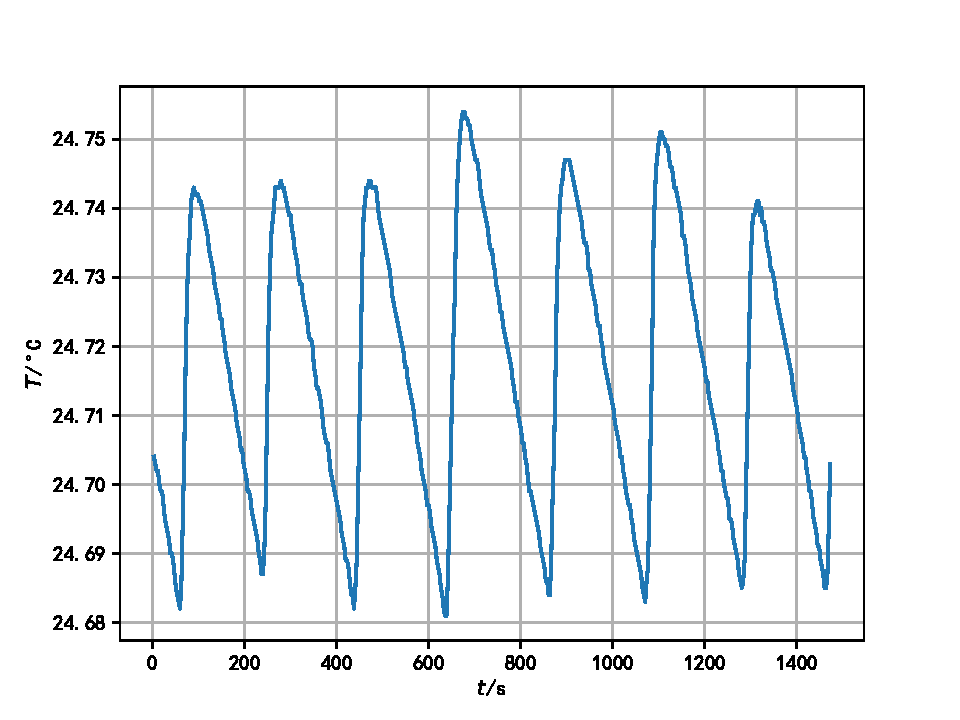
\includegraphics[scale=0.68]{Figure_4.pdf}
    \caption{继电器控制,电压125 V,未通冷却水}
\end{figure}

\begin{figure}[!h]
    \centering
    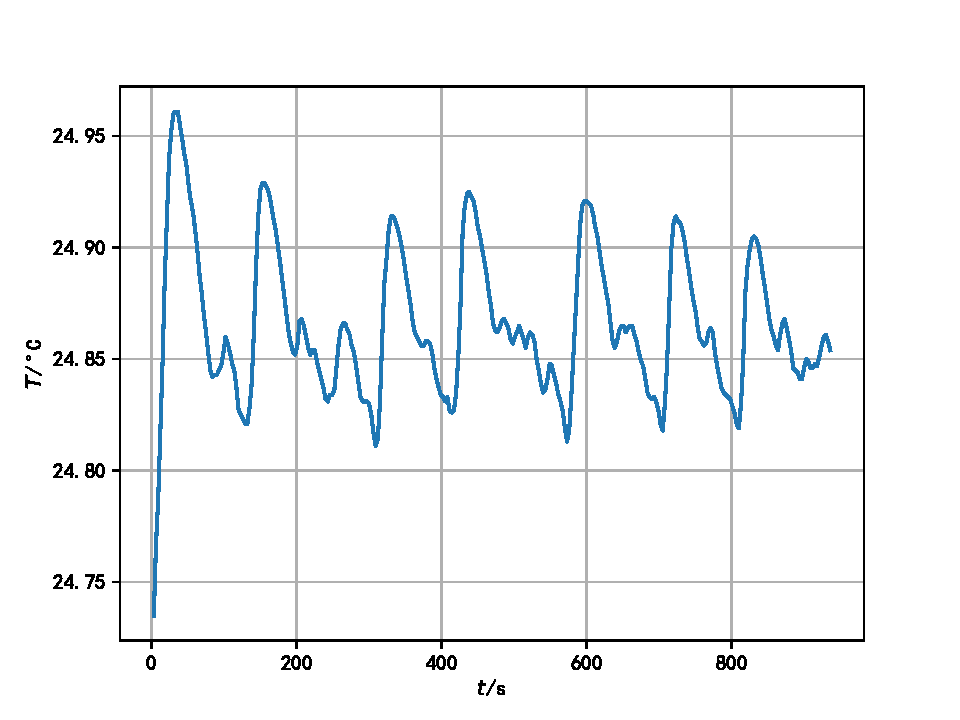
\includegraphics[scale=0.68]{Figure_5.pdf}
    \caption{DTC 控制,电压200 V,通冷却水}
\end{figure}

\begin{figure}[!h]
    \centering
    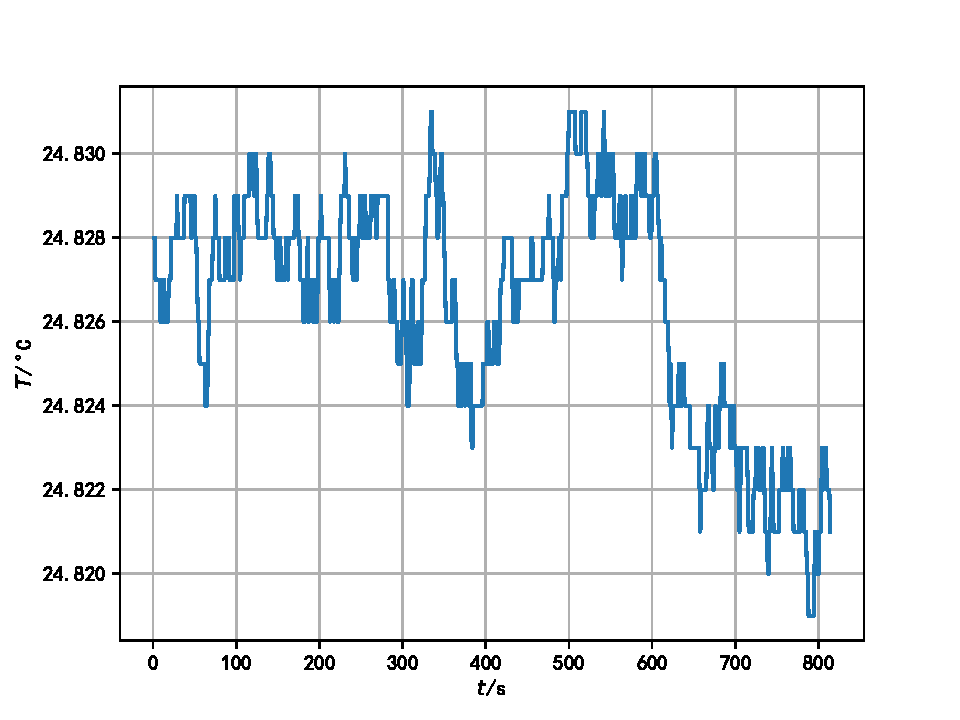
\includegraphics[scale=0.68]{Figure_6.pdf}
    \caption{DTC 控制,电压200 V,未通冷却水}
\end{figure}

\begin{figure}[!h]
    \centering
    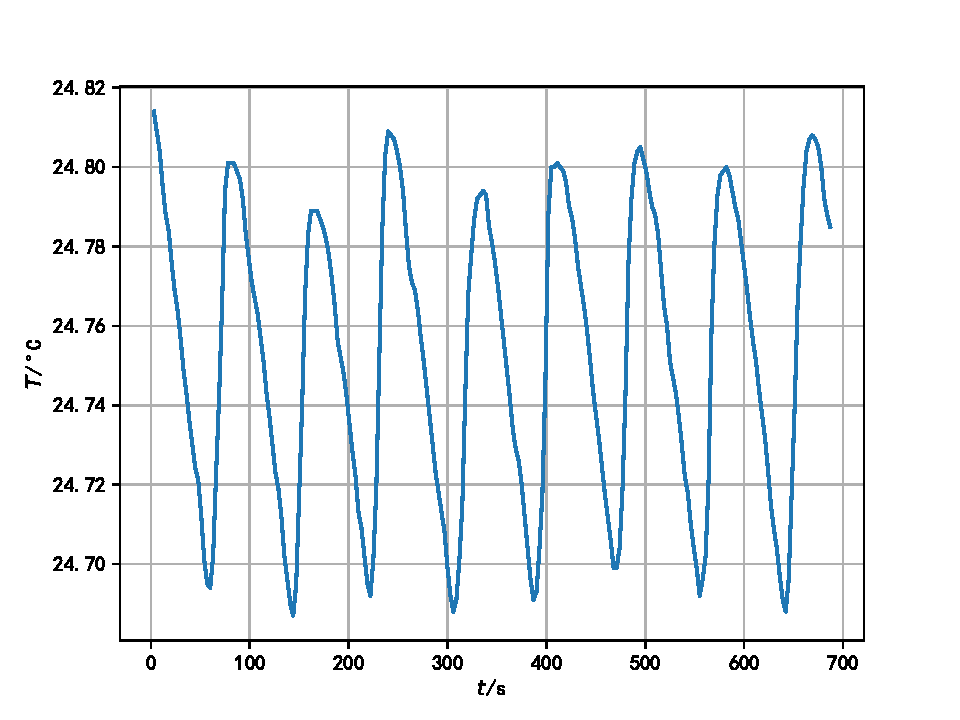
\includegraphics[scale=0.68]{Figure_7.pdf}
    \caption{继电器控制,电压200 V,通冷却水}
\end{figure}

\begin{figure}[!h]
    \centering
    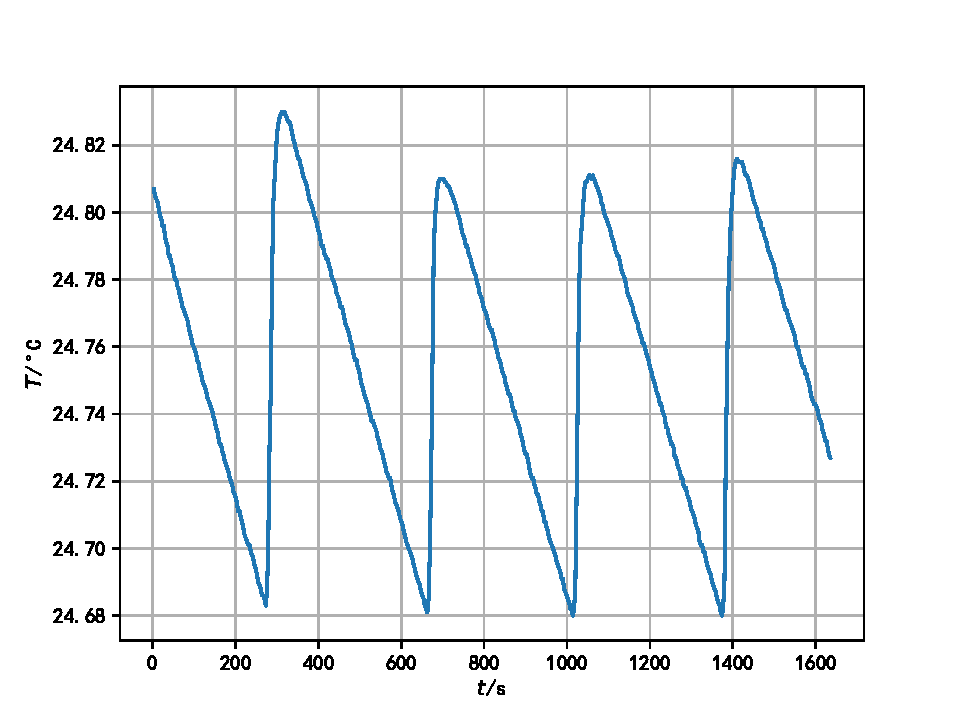
\includegraphics[scale=0.68]{Figure_8.pdf}
    \caption{继电器控制,电压200 V,未通冷却水}
\end{figure}

\pagebreak


\begin{center}
    \Large\bfseries{附件II~~~实验数据截图}
\end{center}

\begin{figure}[ht]
    \centering
    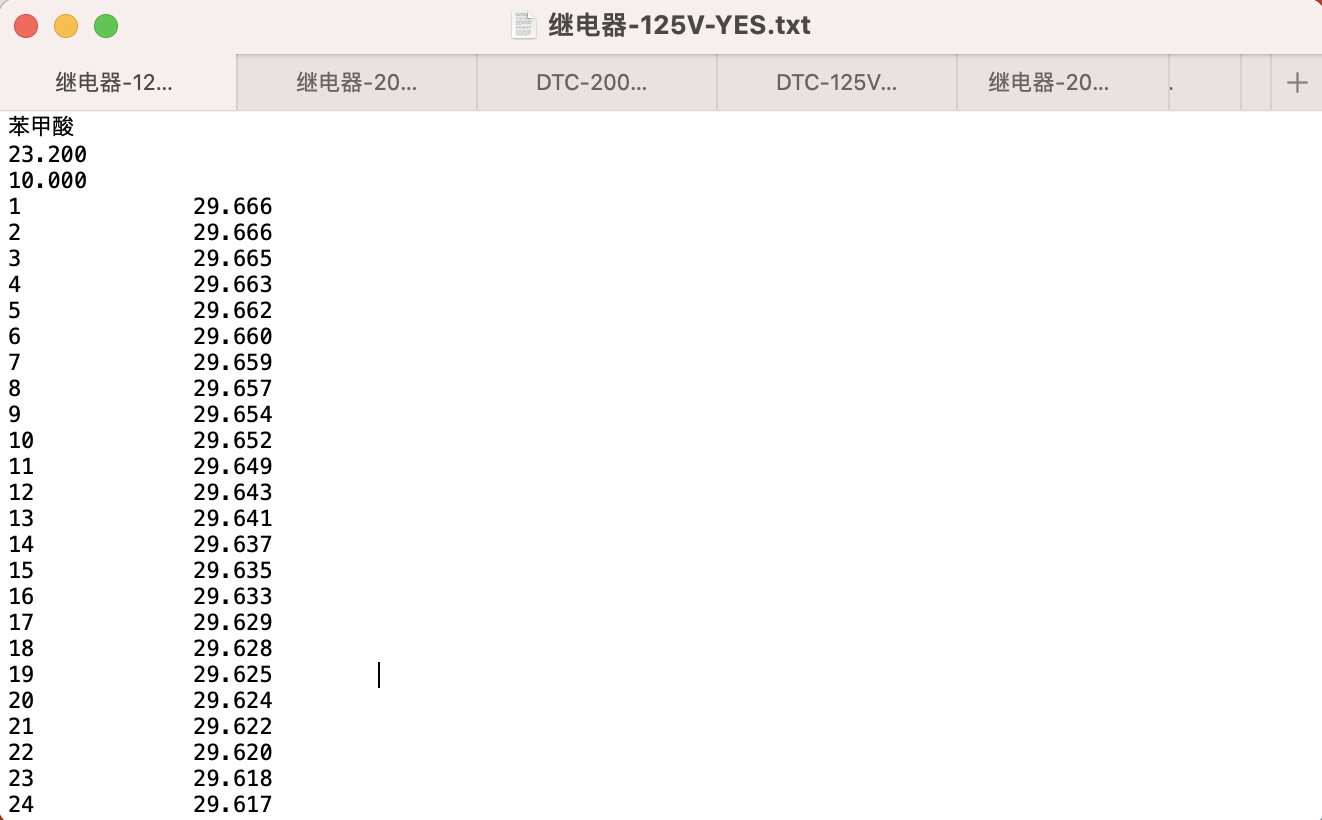
\includegraphics[width=1\textwidth]{1.png}
    \caption{继电器-125V-YES}
\end{figure}

\begin{figure}[ht]
    \centering
    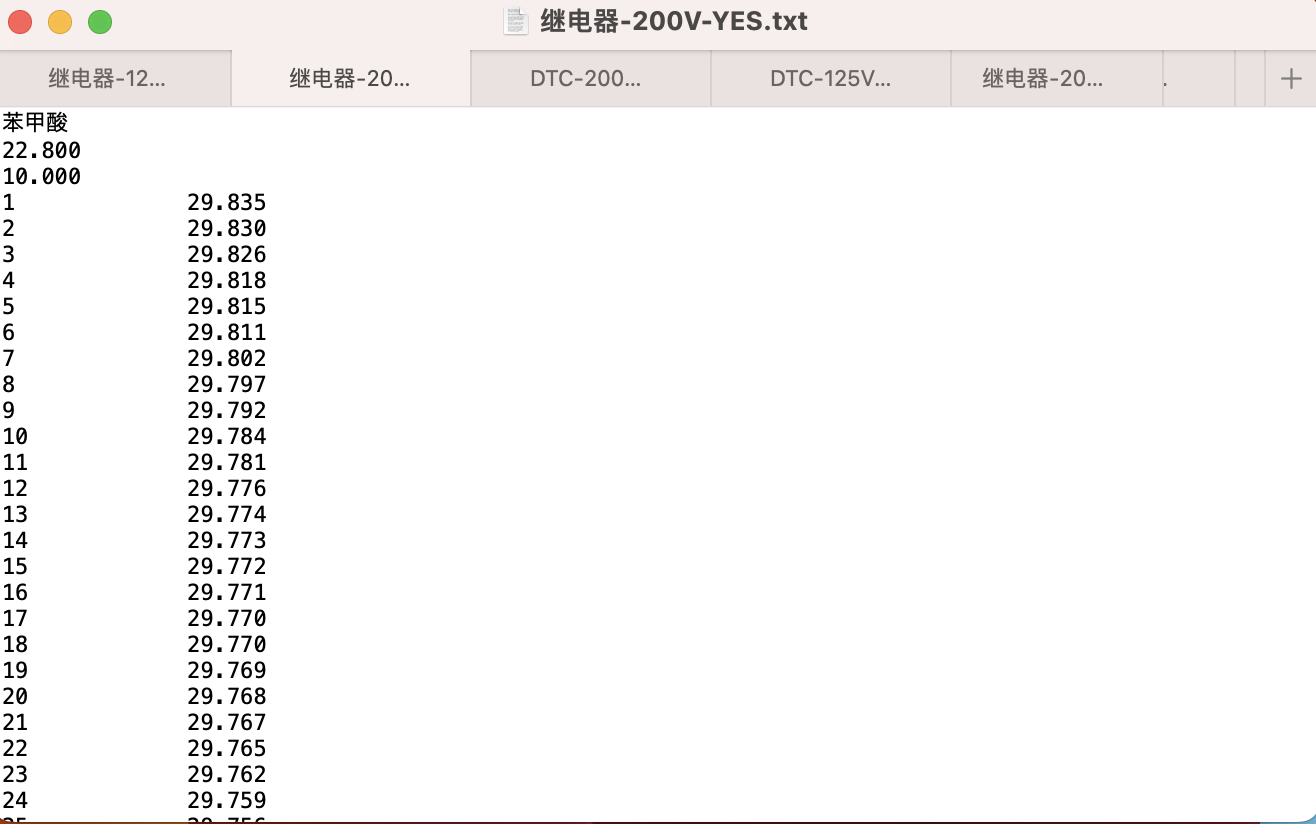
\includegraphics[width=1\textwidth]{2.png}
    \caption{继电器-200V-YES}
\end{figure}

\begin{figure}[ht]
    \centering
    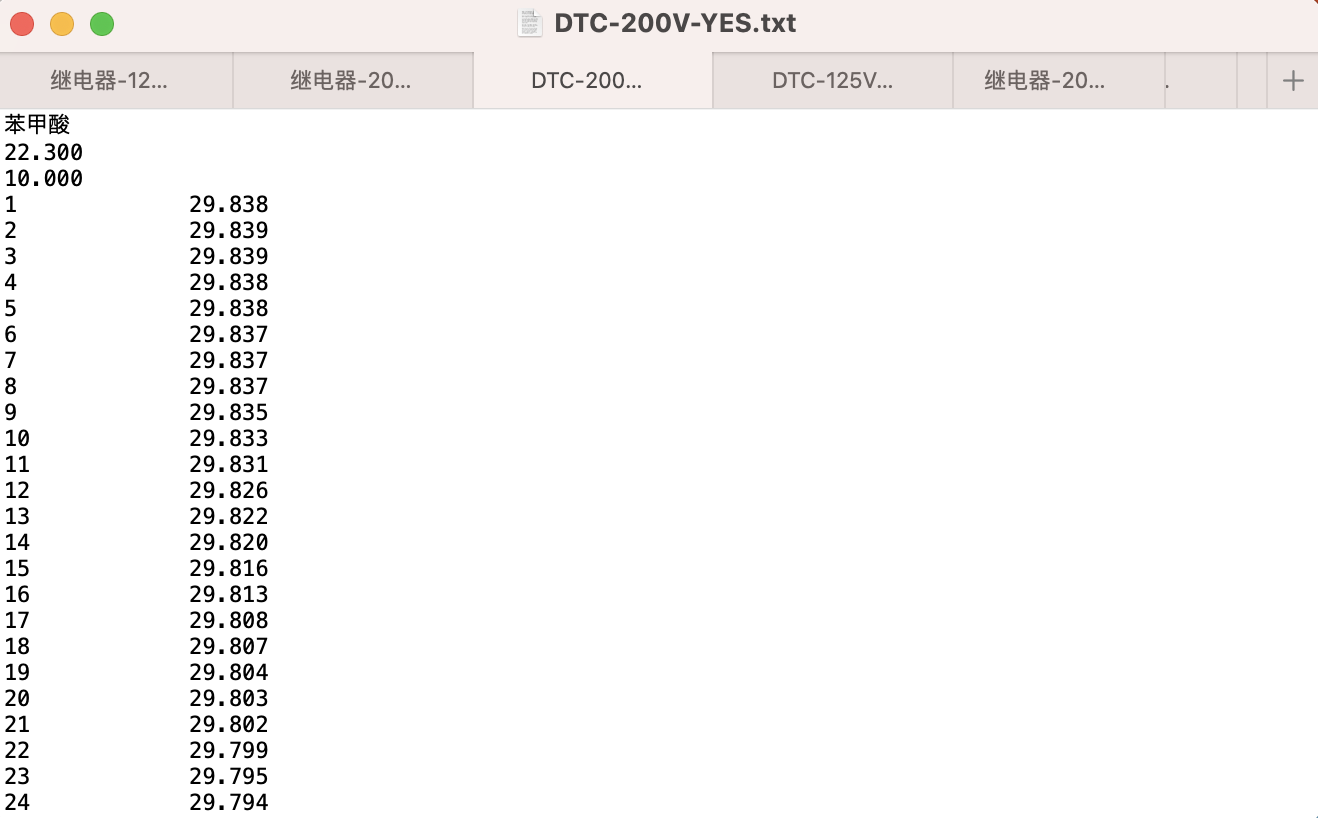
\includegraphics[width=1\textwidth]{3.png}
    \caption{DTC-200V-YES}
\end{figure}

\begin{figure}[ht]
    \centering
    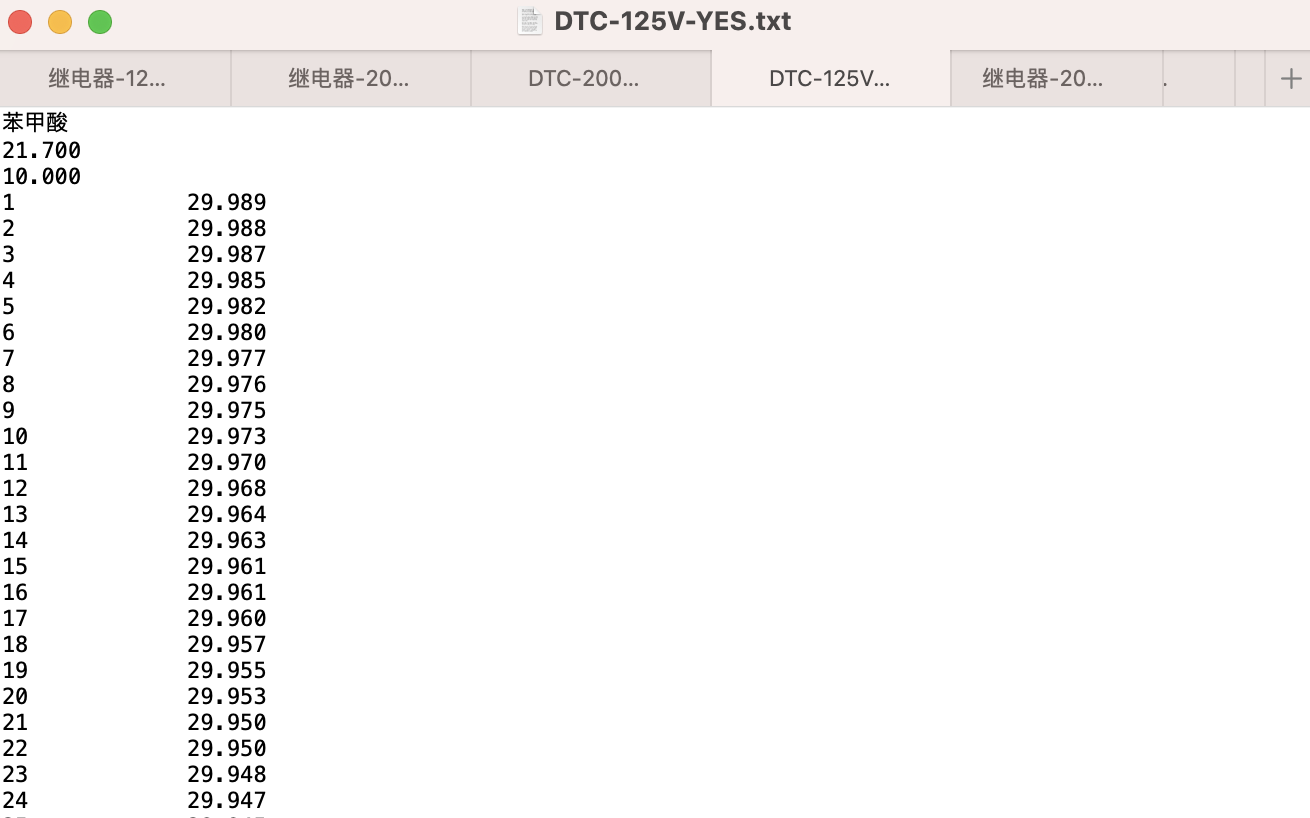
\includegraphics[width=1\textwidth]{4.png}
    \caption{DTC-125V-YES}
\end{figure}

\begin{figure}[ht]
    \centering
    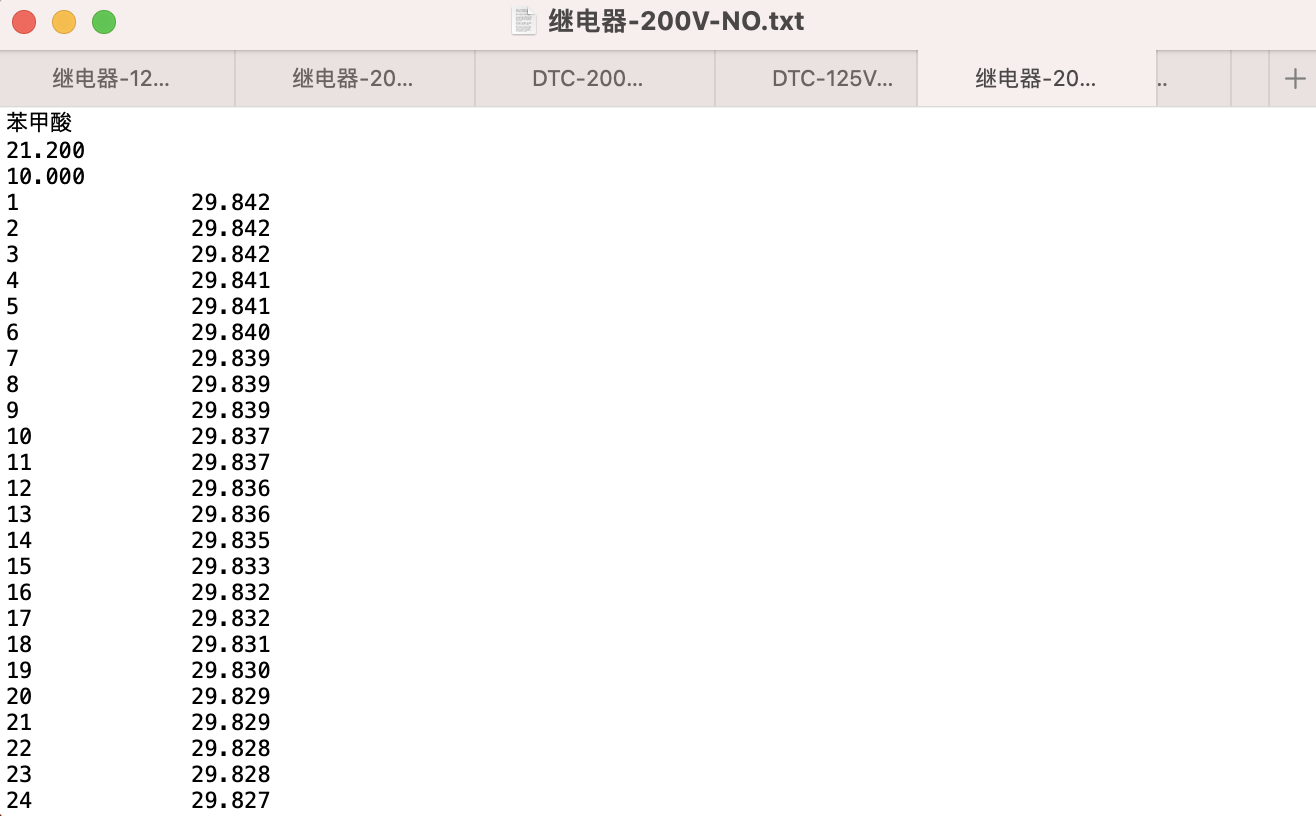
\includegraphics[width=1\textwidth]{5.png}
    \caption{继电器-200V-NO}
\end{figure}

\begin{figure}[ht]
    \centering
    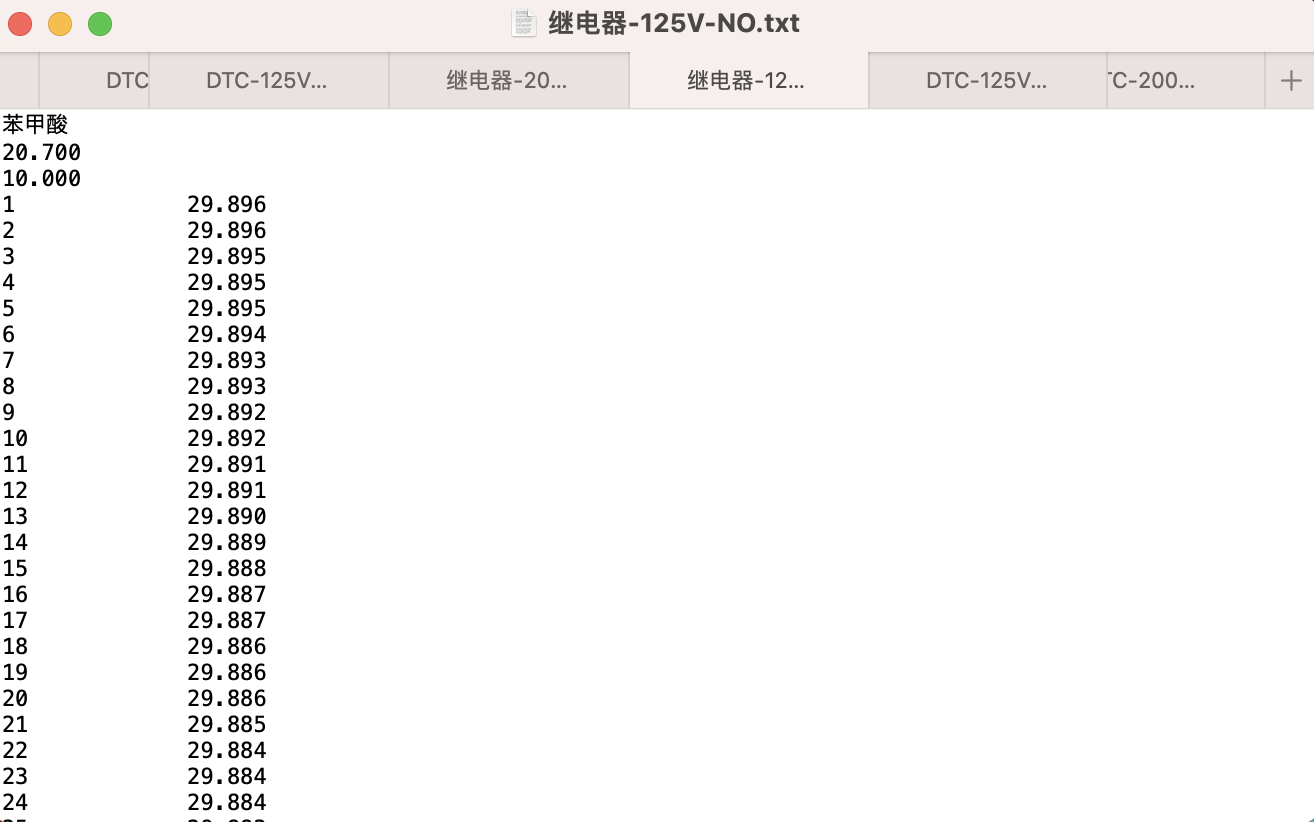
\includegraphics[width=1\textwidth]{6.png}
    \caption{继电器-125V-NO}
\end{figure}

\begin{figure}[ht]
    \centering
    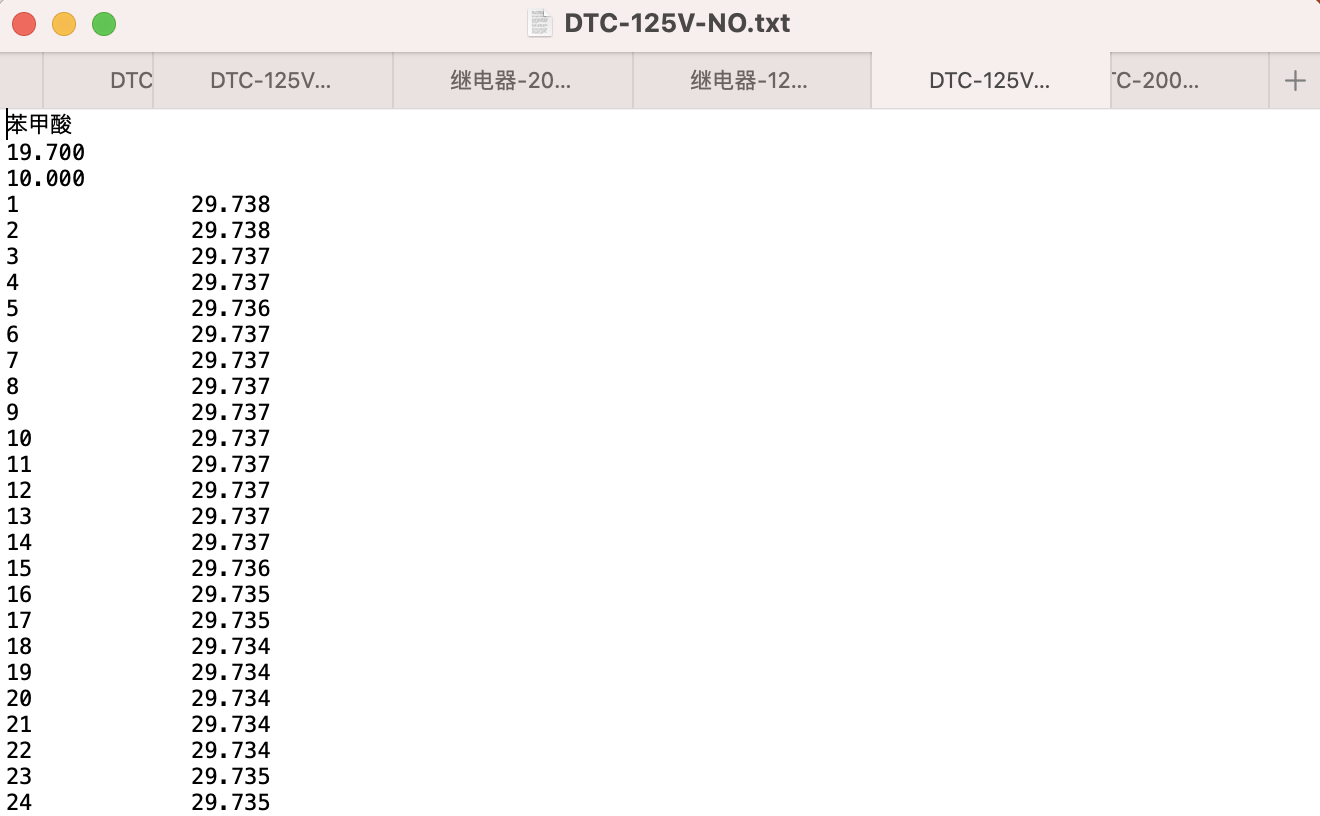
\includegraphics[width=1\textwidth]{7.png}
    \caption{DTC-125V-NO}
\end{figure}

\begin{figure}[ht]
    \centering
    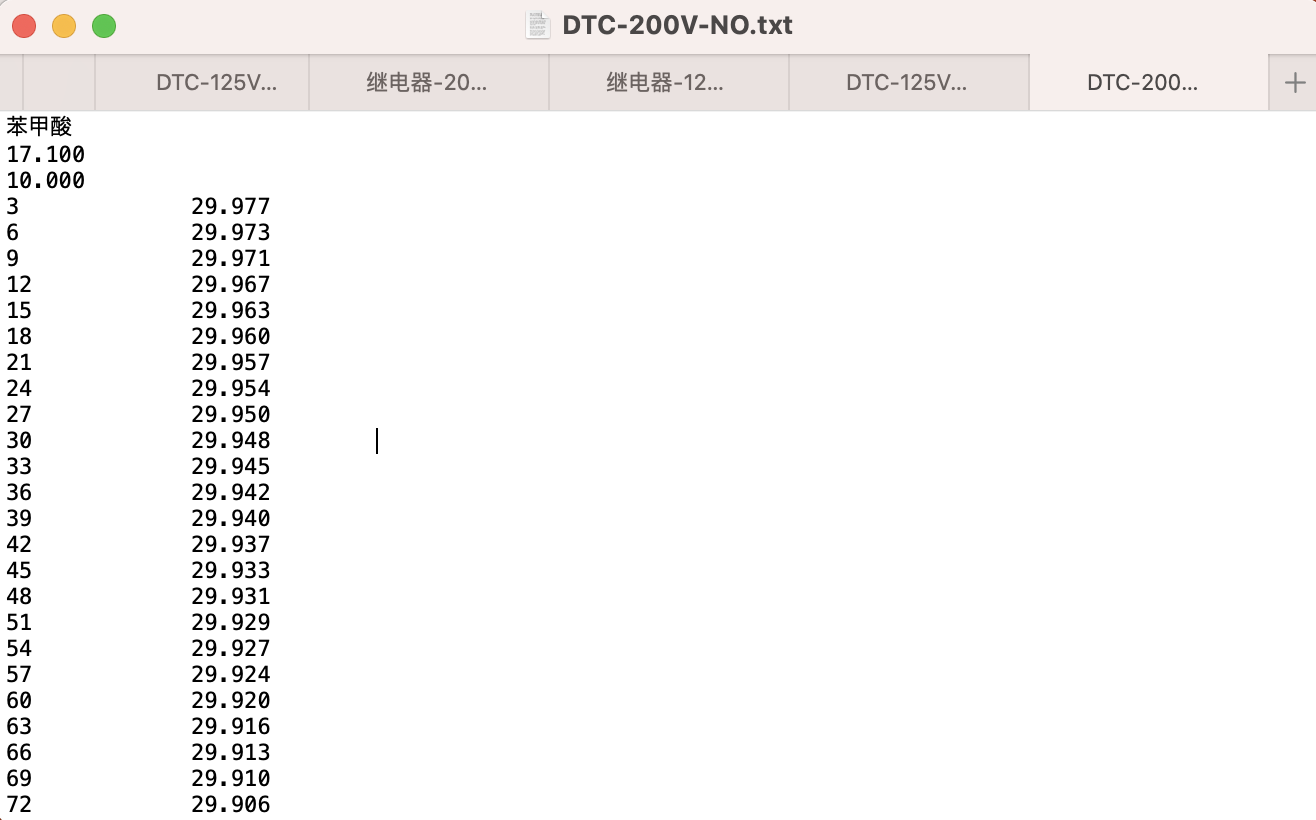
\includegraphics[width=1\textwidth]{8.png}
    \caption{DTC-200V-NO}
\end{figure}

\end{document}
